\documentclass[11pt]{article}
\usepackage[spanish]{babel}
\usepackage[utf8]{inputenc}
\usepackage{listings}
\usepackage{graphicx}
\graphicspath{{../Imagenes/}}

\usepackage[paper=portrait, pagesize]{typearea}
\usepackage{titlepic}

%%% Tablas
\usepackage{tabularx}
\usepackage{float}
\usepackage{adjustbox}
\usepackage{booktabs}
\usepackage{multirow}
\renewcommand{\arraystretch}{1.7}

\begin{document}

\begin{titlepage}
\centering
\vspace{4.5cm}
{\scshape\LARGE Descripción de personajes y escenarios\par}
{\scshape\LARGE Peña de Fútbol\par}
{\scshape\Large Grupo 2.6\par}
\vspace{1.5cm}

{\scshape\large \today \par}
\vspace{14cm}

{Miguel Albertí Pons\\
Sofía Almeida Bruno\\
Pedro Manuel Flores Crespo\\
María Victoria Granados Pozo\\
Lidia Martín Chica
\par}

\end{titlepage}


\newpage

\section{Personajes}
%%TABLA ALBA
\begin{table}[H]
	\centering
	\begin{tabular}{p{0.2\linewidth}|p{0.3\linewidth}p{0.475\linewidth}}
		\toprule
		\textbf{Nombre} & Alba Aguilar Serrano &\multirow{4}{*}{\begin{minipage}{1.\textwidth}
\includegraphics[width=0.2\textwidth, height=30mm]{Alba}\end{minipage}}\\
		\textbf{Edad} & 52 & \\
		\textbf{Sexo} & Mujer & \\
		\textbf{Educación} & Trabaja en una papelería/librería propiedad familiar.  & \\
		\bottomrule
	\end{tabular}
	
	\begin{tabular}{l}
		\textbf{Contexto de uso} 
	\end{tabular}
	
	\begin{tabular}{p{0.2\linewidth}|p{0.8\linewidth}}
		\toprule
		\textbf{Cuándo} & Tras salir de trabajar, ratos libres y/o fines de semana.\\
		\textbf{Dónde}  & Normalmente en casa o en la sede de la peña aunque puede mirarla fuera de estos sitios.\\
		\textbf{Tipo de ordenador} & Teléfono móvil.\\
		\bottomrule
	\end{tabular}
	
	\begin{tabular}{l}
		\textbf{Misión} 
	\end{tabular}
	
	\begin{tabular}{p{0.2\linewidth}|p{0.8\linewidth}}
		\toprule
		\textbf{Objetivo} & Llevar las cuentas de la empresa.
		\\
		\textbf{Expectativas}  & Poder ver el estado de las cuotas de la empresa así como el resto de la contabilidad (alquiler, gastos de comidas, actividades, etc). \\
		\bottomrule
	\end{tabular}
	
	\begin{tabular}{l}
		\textbf{Motivación} 
	\end{tabular}
	
	\begin{tabular}{p{0.2\linewidth}|p{0.8\linewidth}}
		\toprule
		\textbf{Urgencia} & Utilizará la aplicación frecuentemente.\\
		\textbf{Deseo}  & Que el proceso sea fácil y claro para no cometer ningún error.
		 \\
		\bottomrule
	\end{tabular}
	
	\begin{tabular}{p{1.028\linewidth}}
		\textbf{Actitud hacia la tecnología}\\
		\midrule
		Es una persona que no tiene miedo a usar la tecnología ni aprender a utilizar aplicaciones nuevas aunque a veces tenga problemas para entenderlas. Al ser una persona decidida conseguirá realizar todo el proceso.
		
	\end{tabular}
\end{table}

%%TABLA MANUEL
\begin{table}[H]
  \centering
  \begin{tabular}{p{0.2\linewidth}|p{0.3\linewidth}p{0.475\linewidth}}
    \toprule
    \textbf{Nombre} & Manuel Navarro Vázquez &\multirow{4}{*}{\begin{minipage}{1.\textwidth}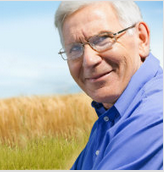
\includegraphics[width=0.2\textwidth, height=30mm]{Pedro}\end{minipage}}\\\\
    \textbf{Edad} & 43 & \\
    \textbf{Sexo} & Hombre & \\
    \textbf{Educación} & Trabaja de policía & \\
    \bottomrule
  \end{tabular}

  \begin{tabular}{l}
    \textbf{Contexto de uso} 
  \end{tabular}
  
  \begin{tabular}{p{0.2\linewidth}|p{0.8\linewidth}}
    \toprule
    \textbf{Cuándo} & Por las mañanas antes de empezar a trabajar\\
    \textbf{Dónde}  & En su casa\\
    \textbf{Tipo de ordenador} & Tiene un móvil no muy moderno\\
    \bottomrule
  \end{tabular}

  \begin{tabular}{l}
    \textbf{Misión} 
  \end{tabular}
  
  \begin{tabular}{p{0.2\linewidth}|p{0.8\linewidth}}
    \toprule
    \textbf{Objetivo} & Subir noticias sobre los equipos a diario, además de informar sobre la organización de los viajes\\
    \textbf{Expectativas}  & Facilidad a la hora de actualizar contenido. Distintas secciones: una para noticias y otra para viajes \\
    \bottomrule
  \end{tabular}

  \begin{tabular}{l}
    \textbf{Motivación} 
  \end{tabular}

  \begin{tabular}{p{0.2\linewidth}|p{0.8\linewidth}}
    \toprule
    \textbf{Urgencia} & Alta, debe poder actualizar la información a diario\\
    \textbf{Deseo}  & Mantener a los aficionados que utilicen la aplicación al día sobre las novedades en este deporte, especialmente las que refieran al Granada. Organizar los viajes de la peña.\\
    \bottomrule
  \end{tabular}

  \begin{tabular}{p{1.028\linewidth}}
    \textbf{Actitud hacia la tecnología}\\
    \midrule
    Utiliza el móvil con facilidad, especialmente las aplicaciones que ya conoce. 
  \end{tabular}
\end{table}

%%TABLA ELENA
\begin{table}[H]
  \centering
  \begin{tabular}{p{0.2\linewidth}|p{0.3\linewidth}p{0.475\linewidth}}
    \toprule
    \textbf{Nombre} & Elena Luzón Pérez  &\multirow{4}{*}{\begin{minipage}{1.\textwidth}
\includegraphics[width=0.2\textwidth, height=30mm]{Elena}\end{minipage}}\\
    \textbf{Edad} & 29 & \\
    \textbf{Sexo} & Mujer & \\
    \textbf{Educación} & Graduada en educación primaria & \\
    \bottomrule
  \end{tabular}

  \begin{tabular}{l}
    \textbf{Contexto de uso} 
  \end{tabular}
  
  \begin{tabular}{p{0.2\linewidth}|p{0.8\linewidth}}
    \toprule
    \textbf{Cuándo} & Al salir del colegio\\
    \textbf{Dónde}  & En el autobús de camino a casa\\
    \textbf{Tipo de ordenador} & Dispositivo móvil\\
    \bottomrule
  \end{tabular}

  \begin{tabular}{l}
    \textbf{Misión} 
  \end{tabular}
  
  \begin{tabular}{p{0.2\linewidth}|p{0.8\linewidth}}
    \toprule
    \textbf{Objetivo} & Usar la aplicación como aficionada\\
    \textbf{Expectativas}  & Estar al día de los resultados de los partidos del equipo y de las noticias \\
    \bottomrule
  \end{tabular}

  \begin{tabular}{l}
    \textbf{Motivación} 
  \end{tabular}

  \begin{tabular}{p{0.2\linewidth}|p{0.8\linewidth}}
    \toprule
    \textbf{Urgencia} & Mínima, cuando tenga interés abrirá la aplicación\\
    \textbf{Deseo}  & Estar informada acerca del equipo de fútbol granadino \\
    \bottomrule
  \end{tabular}

  \begin{tabular}{p{1.028\linewidth}}
    \textbf{Actitud hacia la tecnología}\\
    \midrule
    Se maneja con el móvil y la tablet a nivel de usuario
  \end{tabular}
\end{table}

%%TABLA LAURA
\begin{table}[H]
  \centering
  \begin{tabular}{p{0.2\linewidth}|p{0.3\linewidth}p{0.475\linewidth}}
    \toprule
    \textbf{Nombre} & Laura Martín Chica  &\multirow{4}{*}{\begin{minipage}{1.\textwidth}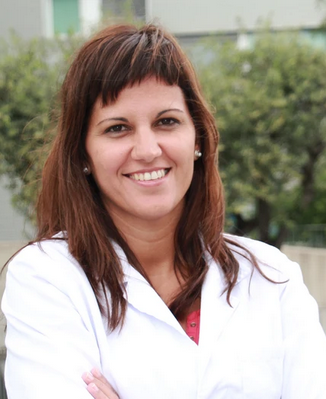
\includegraphics[width=0.2\textwidth, height=30mm]{Ana}\end{minipage}}\\
    \textbf{Edad} & 18 & \\
    \textbf{Sexo} & Mujer & \\
    \textbf{Educación} & Estudiante de Psicología & \\
    \bottomrule
  \end{tabular}

  \begin{tabular}{l}
    \textbf{Contexto de uso} 
  \end{tabular}
  
  \begin{tabular}{p{0.2\linewidth}|p{0.8\linewidth}}
    \toprule
    \textbf{Cuándo} & Siempre que tiene tiempo libre\\
    \textbf{Dónde}  & En su casa\\
    \textbf{Tipo de ordenador} & En este caso, utiliza tanto su portátil como su dispositivo móvil\\
    \bottomrule
  \end{tabular}

  \begin{tabular}{l}
    \textbf{Misión} 
  \end{tabular}
  
  \begin{tabular}{p{0.2\linewidth}|p{0.8\linewidth}}
    \toprule
    \textbf{Objetivo} & Mirar las noticias\\
    \textbf{Expectativas}  & Estar al día de los resultados de los partidos del equipo y de las noticias y poder participar en los viajes para ver jugar a su equipo\\
    \bottomrule
  \end{tabular}

  \begin{tabular}{l}
    \textbf{Motivación} 
  \end{tabular}

  \begin{tabular}{p{0.2\linewidth}|p{0.8\linewidth}}
    \toprule
    \textbf{Urgencia} & Mínima, cuando tenga interés abrirá la aplicación\\
    \textbf{Deseo}  & Encontrar la información que quiere de forma rápida \\
    \bottomrule
  \end{tabular}

  \begin{tabular}{p{1.028\linewidth}}
    \textbf{Actitud hacia la tecnología}\\
    \midrule
    Utiliza con mucha facilidad las aplicaciones para el móvil y el ordenador.
  \end{tabular}
\end{table}

%TABLA ANTONIO
\begin{table}[H]
  \centering
	\begin{tabular}{p{0.2\linewidth}|p{0.3\linewidth}p{0.475\linewidth}}
    \toprule
    \textbf{Nombre} & Antonio Amer Sales &\multirow{4}{*}{\begin{minipage}{1.\textwidth}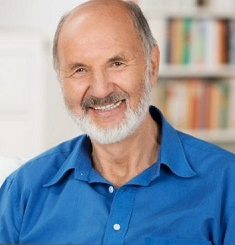
\includegraphics[width=0.2\textwidth, height=30mm]{Antonio}\end{minipage}}\\\\
    \textbf{Edad} & 63 & \\
    \textbf{Sexo} & Hombre & \\
    \textbf{Educación} & Jubilado & \\
    \bottomrule
  \end{tabular}

  \begin{tabular}{l}
    \textbf{Contexto de uso} 
  \end{tabular}
  
  \begin{tabular}{p{0.2\linewidth}|p{0.8\linewidth}}
    \toprule
    \textbf{Cuándo} & Por las mañanas antes después de ir a buscar el periódico\\
    \textbf{Dónde}  & En su casa\\
    \textbf{Tipo de ordenador} & Tiene un ipad\\
    \bottomrule
  \end{tabular}

  \begin{tabular}{l}
    \textbf{Misión} 
  \end{tabular}
  
  \begin{tabular}{p{0.2\linewidth}|p{0.8\linewidth}}
    \toprule
    \textbf{Objetivo} & Ver toda la actualidad del Granada FC \\
    \textbf{Expectativas}  & Facilidad a la hora de ver la última hora y facilidad a la hora de apuntarse a viajes\\
    \bottomrule
  \end{tabular}

  \begin{tabular}{l}
    \textbf{Motivación} 
  \end{tabular}

  \begin{tabular}{p{0.2\linewidth}|p{0.8\linewidth}}
    \toprule
    \textbf{Urgencia} & Alta, debe poder actualizar la información a diario, y las semanas que el Granada FC juegue fuera poder ir.\\
    \textbf{Deseo}  & Poder apuntarse a viajes con gran comodidad.\\
    \bottomrule
  \end{tabular}

  \begin{tabular}{p{1.028\linewidth}}
    \textbf{Actitud hacia la tecnología}\\
    \midrule
    Gracias a la gran pantalla del IPAD le resulta más fácil usar la aplicación.
  \end{tabular}
\end{table}

\section{Escenarios}
%ESCENARIO DE ELENA 1
\begin{table}[H]
  \centering
  \begin{tabular}{p{0.2\linewidth}|p{0.3\linewidth}p{0.475\linewidth}}
    \toprule
    \textbf{Nombre de la persona} & Elena Luzón Pérez &\multirow{2}{*}{\begin{minipage}{1.\textwidth}
\includegraphics[width=0.2\textwidth, height=30mm]{Elena}\end{minipage}}\\
    \textbf{Objetivo persona} & Ver los resultados del partido & \\
    \bottomrule
  \end{tabular}

\begin{tabular}{p{1.028\linewidth}}
  \textbf{Escenario}\\
  \midrule
  Elena es una gran aficionada del club, así que cada vez que sale de trabajar del colegio abre la aplicación, y se pone al día de las noticias que haya sobre el equipo. Además si el día anterior hubo algún partido consulta los resultados.
\end{tabular}
\end{table}

%ESCENARIO DE ELENA 2
\begin{table}[H]
  \centering
  \begin{tabular}{p{0.2\linewidth}|p{0.3\linewidth}p{0.475\linewidth}}
    \toprule
    \textbf{Nombre de la persona} & Elena Luzón Pérez &\multirow{2}{*}{\begin{minipage}{1.\textwidth}
\includegraphics[width=0.2\textwidth, height=30mm]{Elena}\end{minipage}}\\
    \textbf{Objetivo persona} & Darse de alta como socia & \\
    \bottomrule
  \end{tabular}

\begin{tabular}{p{1.028\linewidth}}
  \textbf{Escenario}\\
  \midrule
  Elena cada vez tiene más interés por el club, así que ha decidido hacerse socia, y seguir de cerca al equipo. Para ello abre la aplicación, accede al apartado de registro, introduce sus datos y abona las tasas correspondientes. Finalmente navega por la aplicación como socia. 
\end{tabular}
\end{table}

%ESCENARIO LAURA 1
\begin{table}[H]
  \centering
  \begin{tabular}{p{0.2\linewidth}|p{0.3\linewidth}p{0.475\linewidth}}
    \toprule
    \textbf{Nombre de la persona} & Laura Martín Chica &\multirow{2}{*}{\begin{minipage}{1.\textwidth}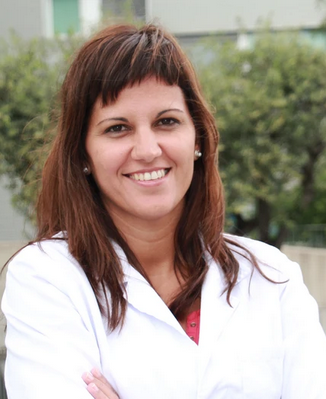
\includegraphics[width=0.2\textwidth, height=30mm]{Ana}\end{minipage}}\\
    \textbf{Objetivo persona} & Ver noticias & \\
    \bottomrule
  \end{tabular}

\begin{tabular}{p{1.028\linewidth}}
  \textbf{Escenario}\\
  \midrule
  Como Laura además de ser abonada, es una gran aficionada al fútbol, le interesan las noticias que puedan aparecer en la aplicación, sobre todo las de tipo deportivo. Como es una persona joven, totalmente habituada al uso de las nuevas tecnologías, le resulta muy fácil encontrar las noticias publicadas y accede con facilidad a las que más le interesan.
\end{tabular}
\end{table}


%ESCENARIO LAURA 2
\begin{table}[H]
  \centering
  \begin{tabular}{p{0.2\linewidth}|p{0.3\linewidth}p{0.475\linewidth}}
    \toprule
    \textbf{Nombre de la persona} & Laura Martín Chica &\multirow{2}{*}{\begin{minipage}{1.\textwidth}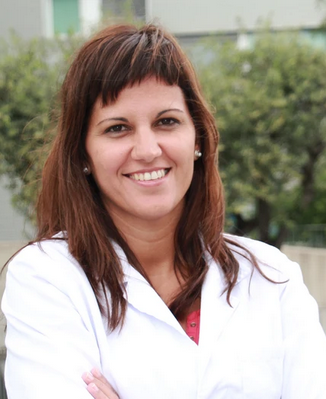
\includegraphics[width=0.2\textwidth, height=30mm]{Ana}\end{minipage}}\\
    \textbf{Objetivo persona} & Apuntarse a un viaje & \\
    \bottomrule
  \end{tabular}

\begin{tabular}{p{1.028\linewidth}}
  \textbf{Escenario}\\
  \midrule
  Este fin de semana, el Granada CF visita uno de los estadios más importantes y complicados de la liga española, el Santiago Bernabeu. Mientras Laura buscaba noticias interesantes, ha encontrado una en la que se informaba a los abonados que es posible realizar un viaje en autobús con entrada incluida, para ver jugar al equipo. Para poder inscribirse al viaje, Laura debe registrarse como abonada para poder reservar la plaza.
Así, de forma rápida Laura está en la lista de abonados que acudirán al partido en autobús. 
\end{tabular}
\end{table}

%ESCENARIO MANUEL
\begin{table}[H]
  \centering
  \begin{tabular}{p{0.2\linewidth}|p{0.3\linewidth}p{0.475\linewidth}}
    \toprule
    \textbf{Nombre de la persona} & Manuel Navarro Vázquez &\multirow{2}{*}{\begin{minipage}{1.\textwidth}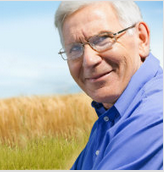
\includegraphics[width=0.2\textwidth, height=30mm]{Pedro}\end{minipage}}\\
    \textbf{Objetivo persona} & Añadir información sobre un viaje & \\
    \bottomrule
  \end{tabular}

\begin{tabular}{p{1.028\linewidth}}
  \textbf{Escenario}\\
  \midrule
  Este fin de semana, el Granada CF visita uno de los estadios más importantes y complicados de la liga española, el Santiago Bernabeu. Con el objetivo de que los socios de la peña puedan mostrar su apoyo al equipo de la forma más cercana, en calidad de directivo, ha decidido organizar un viaje en el que los socios se trasladen hasta la capital. Necesita poder añadir una nueva noticia con toda la información del viaje (fecha, horario, ruta, \dots) en la que, además, los socios puedan reservar su plaza.
\end{tabular}
\end{table}

%ESCENARIO ALBA 1
\begin{table}[H]
	\centering
	\begin{tabular}{p{0.2\linewidth}|p{0.3\linewidth}p{0.475\linewidth}}
		\toprule
		\textbf{Nombre de la persona} & Alba Aguilar Serrano &\multirow{2}{*}{\begin{minipage}{1.\textwidth}
\includegraphics[width=0.2\textwidth, height=30mm]{Alba}\end{minipage}}\\
		\textbf{Objetivo persona} & Consultar si han recibido el pago de un socio.  \\
		\bottomrule
	\end{tabular}
	
	\begin{tabular}{p{1.028\linewidth}}
		\textbf{Escenario}\\
		\midrule
		Alba se encuentra en sede de la peña de fútbol hablando con algunos directivos y amigos de la misma. En un momento se le acerca uno de los Andrés, que se ha hecho socio de la peña recientemente. Le dice, que ha realizado el pago mediante una de las maneras que le explicaron pero que en la aplicación todavía le aparece como que no lo ha realizado. Para ver qué está sucediendo, Alba entra la aplicación. Una vez dentro, accede a la sección donde se encuentran el estado de las cuotas y busca el por el nombre del socio. En su apartado le aparece que está todavía tramitándose y que por eso no le aparece. Alba,para mayor tranquilidad de Andrés, decide avisarle cuando el estado de su pago cambie y así ver si ya está todo correcto. 
	\end{tabular}
\end{table}

%ESCENARIO ALBA 2
\begin{table}[H]
	\centering
	\begin{tabular}{p{0.2\linewidth}|p{0.3\linewidth}p{0.475\linewidth}}
		\toprule
		\textbf{Nombre de la persona} & Alba Aguilar Serrano &\multirow{2}{*}{\begin{minipage}{1.\textwidth}
\includegraphics[width=0.2\textwidth, height=30mm]{Alba}\end{minipage}}\\
		\textbf{Objetivo persona} & Realizar informe de contabilidad. \\
		\bottomrule
	\end{tabular}
	
	\begin{tabular}{p{1.028\linewidth}}
		\textbf{Escenario}\\
		\midrule
		Es final de mes. Como es habitual Alba necesita realizar un informe con todos los gastos y ganancias que ha obtenido la peña en el mes a acabar. Para ello, accede a la aplicación y más concretamente a su sección propia como directiva de cuentas. En ella le aparecen todas las facturas que ha pagado la empresa como gastos de alquiler y luz, los ingresos obtenidos por el pago de cuotas por parte de los socios, etc. Al permitirle la aplicación tener todo ordenado no tarda demasiado tiempo en preparar el informe y salir a tomar algo con sus amigos.
	\end{tabular}
\end{table}

%ESCENARIO ANTONIO
%ESCENARIO Antonio
\begin{table}[H]
  \centering
  \begin{tabular}{p{0.2\linewidth}|p{0.3\linewidth}p{0.475\linewidth}}
    \toprule
    \textbf{Nombre de la persona} & Antonio Amer Sales &\multirow{2}{*}{\begin{minipage}{1.\textwidth}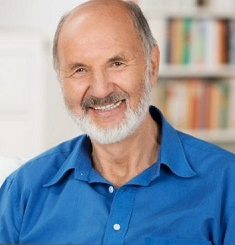
\includegraphics[width=0.2\textwidth, height=30mm]{Antonio}\end{minipage}}\\
    \textbf{Objetivo persona} & Pagar las cuotas & \\
    \bottomrule
  \end{tabular}

\begin{tabular}{p{1.028\linewidth}}
  \textbf{Escenario}\\
  \midrule
  Antonio aún no ha pagado las cuotas del mes de octubre, el administrador le envía un mensaje comunicandole que no está al corriente de los pagos. Antonio al llegar a casa recibe el mensaje del administrador y paga las cuotas.
\end{tabular}

\end{table}

\end{document}
